\documentclass[platex,a4paper,12pt,dvipdfmx]{beamer}
\usetheme{default}
\usepackage{tikz}
\newcommand{\maru}[2]{
%\draw [fill=green,domain=0:360] plot ({#1+#3*cos(\x)},{#2+#3*sin(\x)});
\draw[fill=blue,thick,dotted] (#1) circle[radius=#2];
}

\begin{document}
\begin{frame}{}
  \begin{tikzpicture}
    \draw[help lines] (-5,-5) grid (5,5);
    \only<1>{\maru{1,1}{1}}
    \only<2>{\maru{1,1}{2}}
    \only<3>{\maru{1,1}{3}}
    \only<4>{\maru{1,1}{4}}
  \end{tikzpicture}
\end{frame}
\end{document}